%% LaTeX2e class for student theses
%% sections/content.tex
%% 
%% Karlsruhe Institute of Technology
%% Institute for Program Structures and Data Organization
%% Chair for Software Design and Quality (SDQ)
%%
%% Dr.-Ing. Erik Burger
%% burger@kit.edu
%%
%% Version 1.2, 2016-09-20

\chapter{Theoretical Framework}
\label{ch:theoreticalBackground}

In this chapter, the key elements for understanding the theoretical and experimental work that were developed in this thesis are presented. First, the current state-of-the-art of the integration paradigm is presented; next, the elements used in the integration process for the optical transmitter, the modulator and the photonic wire bond, are presented and described. Finally, the most important figures of merit of the optically packaged transmitted are outlined. 

%\section{Preamble}
%\label{sec:thbkgd:pre}

\section{Integration Process Fundamentals}
\label{sec:thbkgd:fmwk}

%As a preliminary step, a few concepts used in the rest of the document are outlined in the following section. %Note that due to space constraints not all the details about each concept are described in here, but only those considered pertinent for the better comprehension of the rest of the document.

The \textbf{platform} in silicon photonics refers to the substrate of a chip architecture, or photonic component, from which the components are constructed. Monolithic platform integration that supports different photonic components, such as light sources and modulators, is greatly simplified when the same platform is shared between components, and in cases where the platforms are physically incompatible, its reliability and long-term stability are greatly hindered \cite{heteroepiCrumbacker98}. 

Conventional microelectronic circuits are grown and manufactured on a silicon platform, due to the relative mechanical and chemical stability of silicon dioxide as an insulator compared to other semiconductors such as germanium \cite{SiGroFisher12}. Analogically, photonic circuits do not necessarily share the same substrate, since the components have specific requirements in which other semiconductor technologies have better performance, and thus additional steps must be taken in order to connect different optical elements that form the fully integrated device, such as a receiver, an optical amplifier, and of special interest for the present work, a transmitter. %Many of the well-known processes of microelectronic circuits manufacturing are preferably employed in integrated photonics. 

The importance of the type of platform used in integrated photonics resides in the ability to realize optical waveguides and other passive optical elements that allow on-chip light propagation with low losses and strong light confinement, with the advantages of the streamlined processing of silicon \cite{ReedSOI92}. \textbf{Silicon-on-Insulator} (SOI) technology replaces the substrate material from thin silicon films to thin insulator films, such as the key element of SOI, the buried oxide (BOX), due to the improved electric parameters, such as low operating voltage and leak current (reduced conductance); high-speed and high-transmission (reduced junction capacitance); and reduced cross-talk, latch-up and high-resistance supporting substrates (full electrical isolation) \cite{FukudaSOI01}, as well as the expected two-dimensional light confinement \cite{SiPhReed04}.
%such as high power consumption and voltage threshold mismatch (leading to increasing gate leakage) under \SI{45}{\nano\meter}, and the related simplifications in System-on-Chip (SoC) architectures and reliability [citation needed].
%As already mentioned in the introduction, the basic components of an optical transmitter are the laser and the modulator. 
\par \medskip
If heterogeneous platforms are used in the construction of photonic devices, some form of optical integration has to be employed between components which cannot have common embedded waveguides, especially important in the case of non-monolithic components, such as physically separated chips. Such processes are not uncommon in microelectronics and are also known as \textbf{multi-chip packages} (MCM), and they have the function of reducing the packaging wiring for high density chips \cite{PolyWong13}. A straightforward approach for optical connections are free-space optical interconnects, which allow for multiple interconnection paths within a specific optical link, by means of diffractive optics \cite{SiPhPavesi16}. One special challenge of free-space optical interconnect is active alignment, since small perturbations (produced by vibration and temperature drift) can cause beam misalignment and thus, loss of the optical link, and by extent reducing the reliability of the system. \textbf{Photonic wire bonding} (PWB) is a novel technique that provides guided optical interconnection between physically-separated chips, which reduces much of the beam alignment complexity of free-space optical interconnects. 
\par \medskip
Much of the work of the Institute of Photonics and Quantum Electronics has focused in recent years in the optimization and analysis of the photonic wire bond, as seen in the works of Lindenmann \cite{LindenmannPWB12} Petek, \cite{IntPWBPetek16}, Rainer \cite{MMIRainer16}, Onanuga \cite{TapWGOnanuga14} and Pakjović \cite{SOHPajkovic16}, among many others, whose contributions provide the foundation of the present master's thesis. 
%\par \medskip
A brief introduction to optical waveguide structures is given in the following, as they form the basis of most of the optical elements discussed along this master's thesis, including the SOH modulators and the HCSELs. 
%For this thesis project, the substrate material of the lasers is an indium phospide (InP) binary semiconductor featuring a zincblende crystal structure, which can be matched by metal-organic chemical vapor deposition in Si(111) with only partial dislocation of 8\% \ref{Krost_InPSilat93}.
%\lasnotas{talk about the quaternary semiconductors here and then about multiple quantum wells} 
%\lasnotas{talk about HCSELs,why they are fantastic for testing, then about integration}
%Nonetheless, it is more practical to characterize and test the elements of the transmitter separately, and hence using PWB as the linking medium between different platforms comes into play. PWBs are manufactured by a two photon absorption (TPA), a nonlinear process which polymerizes a negative-tone photoresist, allowing for free-form shaping of an optical waveguide linking the two optical elements. The advantage of using PWB over other technologies, such as free form lenses, resides in the ease of characterization and streamlined fabrication. 
%The optical path is analyzed from source to transmission endpoint, meaning that the analysis is started at the laser source, the horizontal cavity surface emitting laser (HCSEL), transmitted through the photonic wire bond (PWB), and modulated at the silicon-organic hybrid (SOH) modulator.
%\lasnotas{add more text about the photonic wirebonds}
%The role of waveguides in photonic integrated circuits (PIC) is the same as copper wires in printed circuit boards: to confine electromagnetic signals and propagate them with low loss among the circuit elements for its manipulation and transmission. Optical waveguides can be single-moded or multi-moded, depending on the type of optical signals they carry, and can be analytically solved through Maxwell's equations, and under certain conditions, simplified due to the properties of the medium they propagate through to the Helmholtz equation. %The analytical solution to optical waveguides is broadly treated by Okamoto \cite{OkamotoWG00} and elsewhere in the literature. %Optical waveguides are the foundation of all the optical elements in the transmitter path, as their structural properties provide information on the fabrication requirements and light confinement required at each stage. 
\subsection{Waveguide Structures}
\label{sec:thbkgd:wg}
The structures of the optical waveguides play a very interesting role in integrated optics, since confinement of waves occurs both in the transverse and the longitudinal directions \cite{SelleriWG15}. For a HCSEL, a \textbf{buried waveguide} provides the light confinement necessary for optical gain and lasing process to occur. for optical modulators, the structure is different since it is preferred to allow for an external electric field to manipulate the optical signal: Such structure is the \textbf{strip-loaded waveguide}, which confines the field between two rib structures physically isolated on each side of the confining slot. This allows for an electrode to be mounted on each side of the waveguide, which in turn is used for generating the modulating electric fields through direct contacting using RF microprobes or electrical wire bonding. The driving voltage is reduced compared to other types of structures because of the long interaction length of the electrode and the waveguide, thus requiring less concentration of modulating electric field to change the phase of the optical waveguide. 

\begin{figure}[!ht]
\centering
  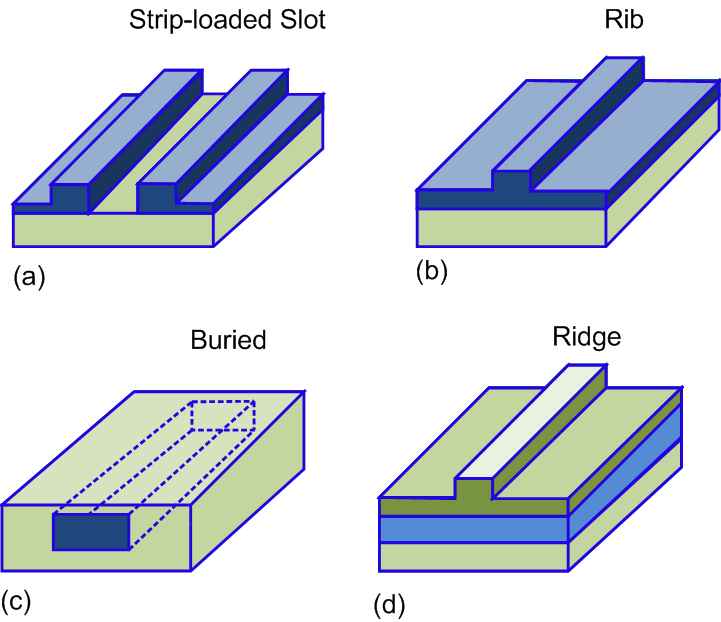
\includegraphics[width=0.6\textwidth]{visio/WGarten}
  \caption{Types of integrated waveguides. (a) strip-loaded slot waveguide, (b) rib waveguide, (c) buried waveguide, (d) ridge waveguide. Blue sections represent the high refractive index portion (guiding region). Adapted from \cite{SelleriWG15}.}
  \label{fig:SelleriWG}
\end{figure}
\par\medskip
As already mentioned, since there is no common substrate between the light source and the modulator, photonic wire bonds allow the optical linking of two optically-independent chips. The creation of free-form optical paths has its own challenges, since the symmetry can no longer be assumed and trajectory-dependent losses have an increasingly important role in the assessment of the insertion loss of the device \cite{ToepferPWB14}. Finally, tapers are used to couple strip-to-slot waveguides by confining the optical fields to a region where the guided modes are coupled with low losses, due to its relative large bandwidth, misalignment tolerance, low facet reflections and robustness required for high performance applications \cite{SPThourhout10} \cite{TapWGOnanuga14}. 

%Losses in an optical waveguide originate from scattering, absorption and radiation.

%\lasnotas{Only some of the following topics will be added depending on which are important for the rest of the thesis. Maybe this is unnecesary}

%More on which platforms are promising in SOH OD
% $\Chi^{2}$ NL, TPA, Spont Emi light
% Waveguides
%MZM/IQ
%Figures of merit BW, Pow, Drive voltage
% Functionalization
% Organic Claddings: DDMEBT 4WM, DFG
 %Basic waveguides:
%	Strip, slot, strip-loaded, double-slot
%field-enhancement: E field discontinuity = interaction b/w mode/cladding
 %Strip: easy fab, low O loss 0.2dB/mm, high drv volt
 %Slot: high conf, low TPA (NLO@pow), diff fab (DUV litho, e-beam), 0.7dB/mm vert OK, hor better alas diff
 %strip ld: EO dev, control cladd E field (enhan). Ideal overlap, low volt; Engi (RF,opti loss). FCA. Elaborate fb. (Difficult design)
 %2xslot: disp eng., ph. match w/ 2nd order NL; DFG, SFG. confined, high NL interact $\chi^2$
% STRIP = EOM!

%Strip-slot-conv:
%	low loss (MultPath Interf) 0.13dB
%	electrodes = separation 
% Log taper

%SOH modulator
% MZ modulator phase shift w/ bias
% phase shift vs. swing%
% IQ modulator (nested modulators)

%\section{Free Carrier Absorption}
%Free carriers can move freely inside a band but they require additional phononic or scattering interactions for momentum conservation \cite{OEDakin06}.

% Electro-optical modulator length , coeff, index changes
%interaction factor $\gamma$
%%%NOT THE SAME AS CONFINEMENT FACTOR!
%%%CONF FACT = Ratio pow in activ sect /tot pow (mode)
%%%INT FACT = Ratio pow(mat+E_field)/tot pow (mode)
%%% INT FACT: only E_x!

%% -------------------
%% | Example content |
%% -------------------




\section{Optical Modulators}

\subsection{Principle of Operation}
In the broadest sense, a signal modulator is a device that mixes a carrier signal $s(t)$, which in the present case is a light source, with a modulation signal $m(t)$ that carries the information of interest. This mixing can be achieved by the electro-absorption or electro-optic effects, and can alter the lightwaves in phase or intensity. %Electro-absorption modulators exploit the absorption edge downshifts towards the forbidden gap due to an external field as first analyzed by Franz and Keldysh \cite{HSphotoDagli07}. 

\begin{figure}[!ht]
\centering
  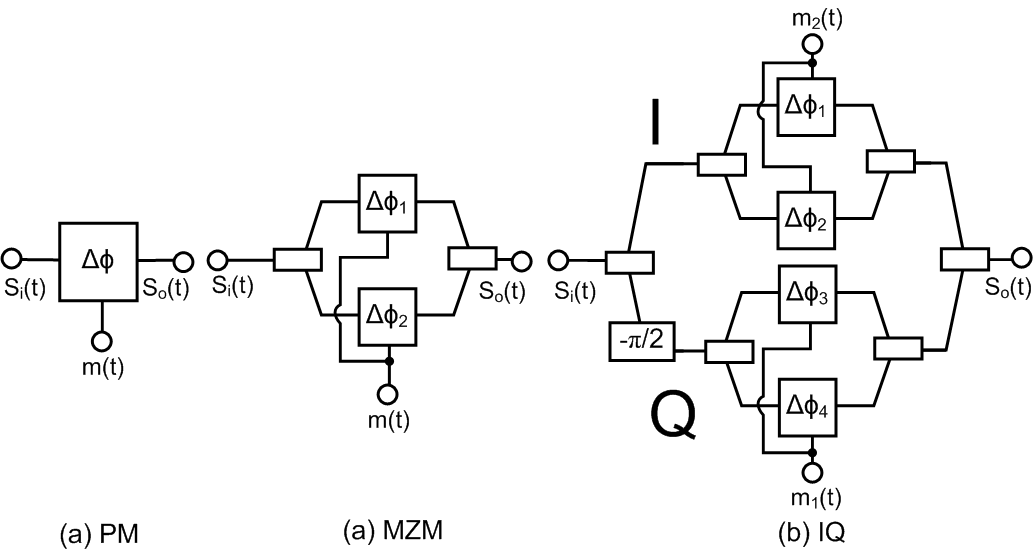
\includegraphics[width=0.8\textwidth]{visio/PM_MZM_IQ}
  \caption{Symbolic representation of different modulator types. (a) shows a phase modulator, (b) shows the Mach-Zender modulator and (c) the quadrature modulator.}
  \label{fig:mods}
\end{figure}

%\emph{phase modulators},
The building blocks for optical modulation are \emph{phase modulators}, \emph{Mach-Zender modulators} and \emph{optical IQ modulators} \cite{SeimetzMod06}. A symbolic representation of each type is shown in figure \ref{fig:mods}. Light is injected to the modulator and split in two equal-power components, and then travel through different optical paths before mixing again at the output. The elements in the optical path will determine the type of the modulator:
%The modulation field overlaps inside the slot and thus transferring the information of the modulation field into the optical field.
\begin{itemize}
\item A phase modulator has an element in the optical path that is controlled by the modulation signal $m(t)$ and induces a relative phase difference $\Delta \phi$ of the output with respect to the input lightwave.
\item A Mach-Zender modulator is made up of two phase modulators where an input wave is split in two different optical paths. Depending on the phase shift introduced on each arm, intensity (or amplitude) modulation can be done on an optical signal, by having constructive or destructive interference at the output of the modulator.
\item A quadrature modulator is made of two MZM in parallel, and features an additional $-\pi/2$ delay for the MZM path in quadrature\footnote{Generally speaking, the quadrature modulator occupies the negative frequencies of the signal spectrum, thus making an efficient usage of the spectral bandwidth.} while the other MZM retains retains the original phase (hence the naming convention \textbf{I}n-phase/\textbf{Q}uadrature). Such configuration allows for different configurations since the carriers of each section are considered orthogonal to each other, and can be used to make better use of the available optical bandwidth.
\end{itemize}

Relative phase difference of the optical signals can be achieved by means of an additional path in one of the arms\footnote{Since the spatial part of the analytical solution of the wave equation reads as $e^{-j\beta z}$, where $\beta$ is the wave vector of the impinging wave.}.One way to achieve a dynamic chance of the path can be achieved by either changing the carrier density of the modulator, or a shift of the refractive index. This can be done by several physical methods: By physical manipulation of the material, such as controlled silicon strain, for instance, nonetheless it requires high voltages to achieve a sufficiently high phase shift. Changing the carrier density through a PN junction or having an electro-optical material which can change its refractive index under an external electric field and thus, leading to a phase change of the optical carrier, are two more efficient methods to produce such optical phase shift. The method that uses plasma dispersion effect\footnote{A change of the real and imaginary parts of the refractive index by means of carrier concentration change\cite{Reedmod05}.}, by using a PIN diode structure around the optical waveguide to alter the density of free carriers, and thus the refractive index and absorption coefficients, are well-known and have been steadily advanced in the literature \cite{ReedSOI14}. However, this implies an inherent nonlinear transfer function which leads to distortion and chirp\cite{LinMZM14}. Integrated optical circuits facilitate the refractive index shift by means of an active electro-optic (EO) material with strong second order non-linearities. An integrated optical phase modulator is based on an optical waveguide in an electro-optic substrate, thus acting as a \textbf{transverse modulator}. An external voltage changes the effective refractive index $n_\text{eff}$ of the waveguide and therefore, the phase of an incoming optical carrier wave. In the Pockels effect regime, the refractive index change can be assumed linear with an external applied voltage across an electrode length $l_\text{el}$:

%The speed of the device depends on the materials used in its fabrication.  %seems like a random out-of nowhere comment in here

%The optical carrier phase can be
%\lasnotas{this needs to be changed around to accomodate for modulation by either method and then introduce SOH.}

\begin{align}
\phi_\text{PM}(t) = \frac{2\pi}{\lambda} \cdot \Delta n_\text{eff} \cdot l_\text{el} \approx u(t)
\end{align}

The necessary voltage for achieving a phase shift of $\pi$ between the two arms is denoted as $V_\pi$. The transfer function\footnote{The ratio of the input and output of an optical modulator.} for single-arm drive is expressed as:

\begin{align}
\frac{s_o(t)}{s_i(t)} = TF(t) = \exp \left( {j\frac{u(t)}{V_{\pi}}\pi} \right)
\end{align}

Where $s_o(t)$ is the output signal and $s_i(t)$ is the input signal. Interference between waves can be exploited for intensity modulation. In other words, the carrier can be turned on (constructive interference) and off (destructive interference) by using two phase modulators being driven by voltages of the same magnitude but equal (or opposite) signs, respectively. This is referred to as a \textbf{push-pull Mach-Zender modulator}. In this configuration, chirp-free amplitude modulation is achieved (because the phase of both arms is preserved at the output) or \emph{balanced} configuration. The transfer function in the push-pull case $TF_\text{PP-MZM}(t)$ can be reduced in this case to: %The transfer function for the DD-MZM for $V_\pi$ phase shift is therefore
%\begin{align}
%TF_\text{DD-MZM}(t) = \frac{1}{2} \cdot \left( e^{j\frac{u(t)}{V_{\pi_1}}\pi} + e^{j\frac{u(t)}{V_{\pi_2}}\pi} \right)
%\end{align}

%\begin{align}
%TF_\text{DD-MZM}(t) = \frac{1}{2} \cdot \left[\exp \left( {j\frac{u_1(t)}{V_{\pi_1}}\pi} \right) + \exp \left( {j\frac{u_2(t)}%{V_{\pi_2}}\pi} \right) \right]
%\end{align}

%For simplification, the $V_\pi$ on both arms will be set to a single value ($V_{\pi_1} = V_{\pi_2} = V_\pi$) %what is the name when you have the same to the left and the right bleh




\begin{align}
TF_\text{PP-MZM}(t) = \cos \left( \frac{\Delta \phi_\text{MZM}(t)}{2} \right) = \cos \left( {j\frac{u(t)}{V_{\pi}}\pi} \right)
\end{align}

The transfer function for power and field can be observed in figure \ref{fig:TF}. The operating point can be chosen at the quadrature point ($V_\pi$, half power transmission, or \SI{3}{\decibel} point, allowing for maximum swing) or at minimum (or maximum) transmission point. If modulation voltage swing is larger than $V_\pi$, it can be seen that there is no significant effect in the transfer function, and thus \emph{overmodulation} occurs \cite{SaeckingerMZM09}. 
%\cite{OptiCommNguyen09}
\begin{figure}[!ht]
\centering
  \includestandalone[width=0.6\textwidth]{tikz/TF}
  \caption{Generalized transfer function for field and power. The power transfer function is cosine-shaped and has the null point at $V_\pi$ or half-wave bias voltage, which is the voltage required to shift the input by $\pi$ at the output port. This point also provides the most linear transfer characteristic and thus its importance in MZM optical characterization.}
  \label{fig:TF}
\end{figure}

\begin{figure}[!ht]
\centering
  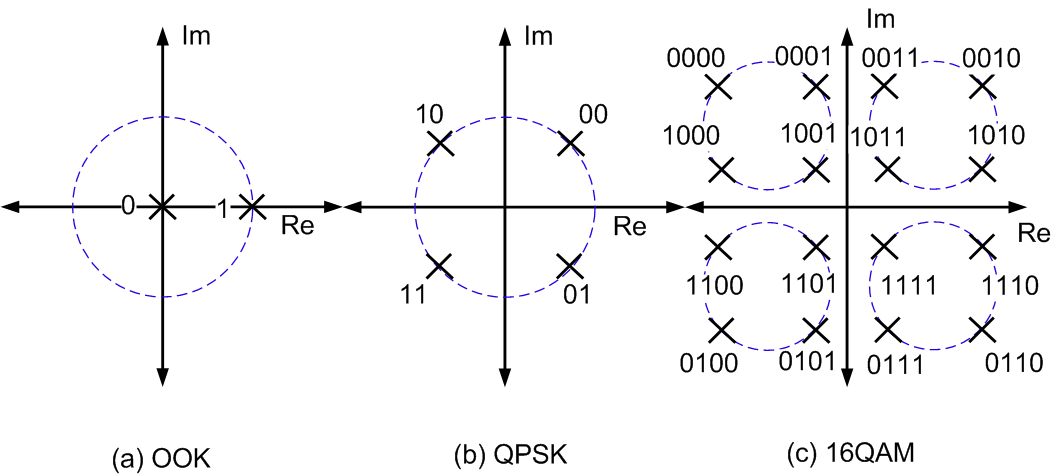
\includegraphics[width=0.8\textwidth]{visio/mod_formats}
  \caption{Modulation formats. (a) shows On-off keying (OOK), which can be achieved by simply turning the carrier signal on and off, such as in a MZM. (b) and (c) show quadrature phase shift keying (QPSK) and seno-denary quadrature amplitude modulation, or 16QAM, which use IQ modulators to achieve the data constellation observed in the figure.}
  \label{fig:mod}
\end{figure}

Finally, the modulation formats that are used in this work are shown in \ref{fig:mod}. The simplest modulation format, on-off keying, can be done simply by using a MZM and modulate the amplitude of the carrier. The other two formats exploit the orthogonality obtained in the arms of the IQ modulator and achieve different constellations in the phase diagram that correspond to a different binary value, in this case a 16-bit symbol. 

%An optical carrier is intensity modulated by an RF signal with an MZM biased at quadrature \cite{LeeMZM06}. 

Several figures of merit can be obtained from Mach-Zender modulators which provide a reference for the performance. All modulators present a periodic \textbf{free spectral range} (FSR) which occurs when the constructive and destructive interference at the output reach their maximum value, and so the maximum and minimum transmission is observed. This also provides information on the \textbf{extinction ratio}, which gives the dynamic range of a modulator (i.e. the intensity difference between maximum and minimum transmission), as a function of the effective additional distance traveled by a wave inside the modulator (large path length difference leads to small FSR). It is common in the literature to see these modulators referred to as unbalanced (i.e. optical path imbalance) and balanced (i.e. equal optical paths on both arms). The differential delay of a Mach Zender interferometer can be calculated from the free spectral range as $\text{FSR}=1/\tau$. As mentioned before, $\text{V}_\pi$ also provides information of the first zero of the power transfer function of the MZM, i.e. the linear region operation, which is preferably low in order to use low power for driving the device. Since there is a change of the refractive index of the electro-optical material, phase matching can be of great importance if there is a slight variation of the phase in one of the arms. The bias point of the modulator can be thus shifted to allow for maximum (or minimum) transmission in each arm of the modulator, or for jitter control by using an embedded thermal phase shifter that operates on the basis of a resistor on top of a waveguide that produces an optical phase shift in one on the arms based on Joule heating.

%For most cases, the modulator is considered \textbf{balanced} if the phase between the two arms of the MZM are of equal length. If a length variation is introduced in one of the arms, one can refer to the modulator as \textbf{unbalanced}, which can be corrected if one of the arms can be independently biased to match the phase on both arms. 



%A Novel Measurement Approach for the Half-wave Voltage
%of Phase Modulator based on PM-MZI Photonic Link
%Li Xianghua, Yang Chun*, Ye Quanyi, Chong Yuhua, and Zhou Zhenghua

\subsection{Electro-Optic Effect}
%$\textbf{\epsilon}(\omega)$
The electro-optic effects correspond to the change of the refractive index or absorption coefficient of a material, $\Delta n$ and $\Delta \alpha$, respectively, due to an external electric field. The quantities are closely related through the Kramers-Kronig relations \cite{OEDakin06}. Changes in the refractive index are modeled through the dielectric function $\mathbf{\epsilon}(\omega)$ of the material. From Maxwell's constitutive equations it is known that the displacement vector $\underline{\textbf{D}}$ in an anisotropic medium is proportional to the electric field by $\underline {\mathbf{E}} = \frac{1}{\epsilon_0} \underline{\mathbf{\eta}} \underline{\mathbf{D}}$ in a form that is convenient to represent the \textbf{dielectric impermeability tensor} $\underline{\mathbf{\eta}}= (\epsilon_0 \underline{\mathbf{\epsilon}}_r)^{-1}$. This is widely studied by the field of crystal optics, with the impermeability tensor expanded around $\mathbf{E}=0$ leading to the linear and quadratic electro-optic effects \cite{PhotoSaleh91} as:
%$\underline D = \underline\epsilon_0 \underline\epsilon_r \underline E$



%\begin{align}
%\eta_{ij} (\mathbf{E}) = \eta_{ij} + \sum_k r_{ijk} E_k + \sum_{kl} s_{ijkl} E_k E_l, \qquad i,j,k,l=1,2,3
% \end{align}

\begin{align}
\underline \eta_{ij} (\mathbf{E}) = \eta_{ij} + \sum_k \underline r_{ijk} E_k + \sum_{kl} \underline s_{ijkl} E_k E_l, \qquad i,j,k,l=1,2,3
 \end{align}

Since the dielectric impermeability tensor is proportional to the inverse of the square of the refractive index, the \textbf{electro-optic tensor} $\underline{\mathbf{r}}_{ijk}$ is usually used in the literature to describe the strength of the impermeability tensor under an external field. Due to inherent crystal symmetries \cite{BoydNLO08}, many of the tensor components vanish, leading in anisotropic crystals to strongly preferential $r_{33}$, $r_{13}$ and $r_{63}$ coefficients, depending on which orientation the material of interest is used. For uniaxial crystals, if an optical wave propagates through a crystal of length $L$, the normal modes experience a phase delay $\Delta \varphi = r_{63}n_o^3E_z k_0 L = r_{63}n_o^3 k_0 U$. This configuration is known as a \textbf{Pockels cell}. 

%A reduced electrode length results in a lumped capacitance that limits the bandwidth to approximately \SI{1}{\giga\hertz}, with modulator lengths in the centimeter range. 
%The fabrication of \ce{LiNbO3} wafers can be done by indiffusion in metals \cite{WootenLiNBo300} and can be cut in different directions depending on the applications. In order to achieve larger transmission speeds, ridge waveguides must be used since they confine the electric field in the waveguide better and confines the optical mode more tightly; the challenge in ridge waveguides made from \ce{LiNbO3} relies on the etching and directionality of the waveguide, which in turn determines the confinement quality and thus the losses of the modulator.
The most prominent inorganic material used for optical modulators is lithium niobate, also known as \ce{LiNbO3}, which has been enabled for low driving voltage, low drift and bias-free operation, as well as optical transparency and high electro-optic coefficients \cite{WootenLiNBo300}. A significant disadvantage of \ce{LiNbO3} modulators is that large voltages or long interaction lengths (by means of the electrode length) are required for efficient modulation, thus the figure of merit $V_\pi L$ provides information of the switching capacity of the modulator per unit length. The $r_{33}$ value of \ce{LiNbO3} is \SI{32.2}{\pico\meter/\volt} at \SI{632.8}{\nano\meter}  \cite{BosshardOrgaNLO95}. This provides a good rule of thumb for the expected value in organic compounds, at optical telecommunication wavelengths (\SI{1.3}{\micro\meter} and \SI{1.55}{\micro\meter}), such as SEO100 and SEO250, produced by Luxtera, that have reported $r_{33}$ values of \SI{160}{\pico\meter/\volt}  and \SI{250}{\pico\meter/\volt} \cite{HerreraSEO12} \cite{JouaneSEO14}. Thus it can be seen directly from these that the required driving voltage of a SOH modulator is significantly lower than that of inorganic material, as well as a smaller footprint.

%1. O. Herrera, “Nonlinear Photonics in Waveguides for Telecommunications”, Ph.D. Dissertation, College of Optical Sciences, University of Arizona (2014)
%Y. Jouane, Y-C. Chang, D. Zhang, J. Luo, A. K-Y. Jen, and Y. Enami, “Unprecedented Highest Electro-Optic Coefficient of 226 pm/V for Electro-Optic Polymer/TiO2 Multilayer Slot Waveguide Modulators”, Optics Express, DOI:10.1364/OE.22.027725, (2014)




\subsection{Silicon-Organic Hybrid Modulators}

%LinBO3: photorefractive effect: electrons ionized impurities excited to CB, charge separation, local e field,delta EO effect 
%equivalent resitance due to molduation: conductivity in buffer and EO material. Resistivity control of buffer and match to WG layer before deposition!

%Independent LiNBO3: Anisotropy. TE/TM mode coupling with off diagonal elements of electro optial tensor. Require special crystam cuts and electrode geometries. Not for high speed

At the core of the silicon-organic hybrid (SOH) Mach-Zender modulator (MZM) there are two SOH phase modulators, which consist of a slot waveguide covered by an organic electro-optic material, that are driven in push-pull mode by a single coplanar transmission line in ground-signal-ground (GSG) configuration \cite{Koos_SOH2015}. 

\begin{figure}[!ht]
\centering
  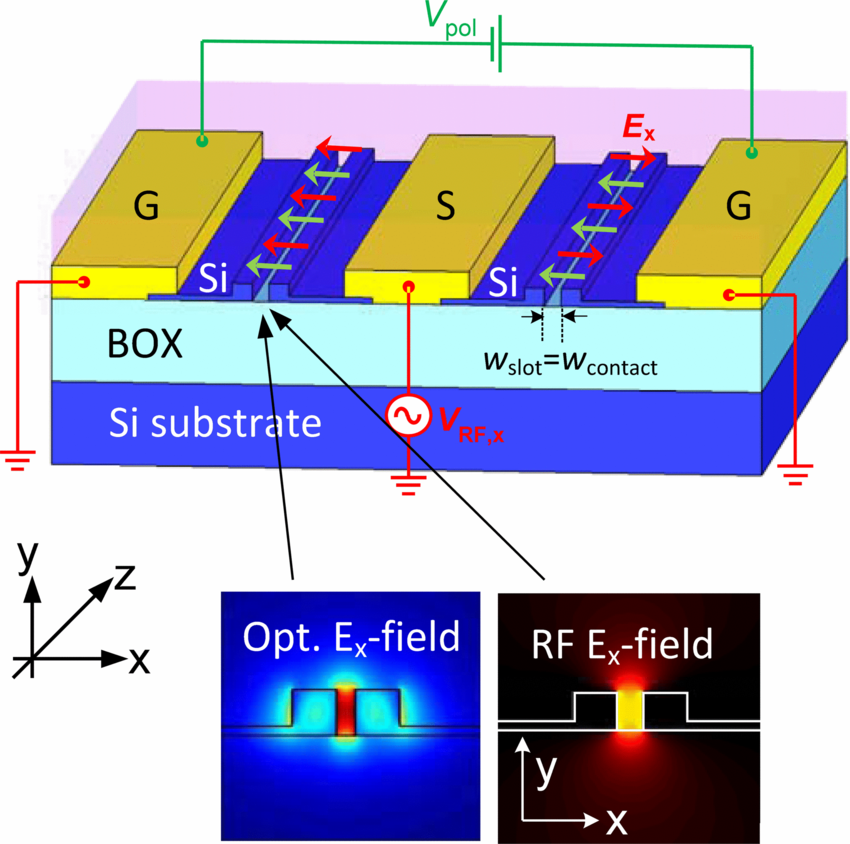
\includegraphics[width=0.7\textwidth]{figs/striploadedWG}
  \caption{Schematic cross section of an SOH MZM showing Si strip-loaded slot waveguides. Two slot waveguide phase modulators, driven in push-pull operation by a single coplanar ground-signal-ground transmission line. The signal is split and combined between the two arms using a multimode interferometer (MMI). The slots are filled with an electro-optic polymer which is poled in a previous step with a voltage $V_\text{pol}$. Below, the simulation of the interacting optical and RF field are shown, showing the strong overlap in the slot region. Adapted from \cite{Koos_SOH2015}.}
  \label{fig:striploadedWG}
\end{figure}

The \textbf{silicon-organic hybrid} (SOH) platform incorporation of organic compounds extend and improve the functionalities that cannot be achieved by silicon alone, and yields a very large amount possible engineering solutions to cater to fully integrated solutions \cite{SOHPICKorn13}. Organic compounds are usually used as the cladding, since the wave interaction that exploits the Pockels effect occurs inside the waveguide slot. The modulating field leads to an ultrafast electro-optic effect with high field overlap, since the modulating field and the carrier are confined inside a very narrow space \cite{gateAlloatti12}. Since the field overlap is very high, the required voltage for strong phase shift is lower than \SI{1}{\volt}. A more detailed schematic description of the physical implementation of the SOH MZM is described in figure \ref{fig:SOHMZMsch}.

\begin{figure}[!ht]
\centering
  \includestandalone[width=0.7\textwidth]{tikz/mzm}
  \caption{Schematic representation of a Mach-Zender modulator (MZM). An input lightwave is split in two equal-power branches by an MMI-based beam splitter, and then converted to an adequate mode field by strip-to-slot converters. An EO polymer is deposited inside the slot waveguides and interacts with the incoming lightwave inside it by an external RF field. The mode fields are re-converted for strip waveguide propagation and recombined in an MMI-based combiner. Adapted from \cite{Koos_SOH2015}.}
  \label{fig:SOHMZMsch}
\end{figure}

The laser light is injected through the input node. For branching the laser light a multimode interferometer (MMI) is used, which is a multimode waveguide optical branch used to split the power into the two arms of the MZM. The preference of MMI for branching power resides on having a simple structure (so there is no need to have an additional structure coupler); large optical bandwidth; polarization insensitivity (as birefringence correction can be used \cite{XipolMMI07}); and robustness against fabrication tolerances \cite{SoldanoMMI95}.

As discussed in the work of Soldano \cite{SoldanoMMI95} and Bachmann \cite{BachmannMMI94}, an MMI can be analyzed through the effective refractive index method to decrease the dimensionality of a 3D problem to 2D. To obtain a 2x2 MMI coupler, and therefore 2 non-mirrored, real images\footnote{Mirroring occurs due to the odd symmetry of the interference, and the real image is also noted because a virtual image is projected into the half-plane $x<0$, but that proves unnecessary for real devices where only forward waves are analyzed.} of a single input field, it is sufficient to have a propagation distance of $z=3L_\pi /2$, which for optical communication yields a value of $\SI{23.5}{\micro\meter} \times \SI{4.5}{\micro\meter}$\footnote{Taken from direct measurement of layout in the IME05 chip}. The same structure would result in constructive interference in one port when mixing the modulated waves incoming from the Mach-Zender interferometer.

%\lasnotas{For this derivation: remember power coupling efficienty for vectorial and scalar fields, mode scalar expansion of a dominant transverse field, itno guided and radiation modes, $\Phi$ is the excitation field, $\Psi$ is the guided mode field or mode field expansion, far from cutoff, resonance condition, $L_\pi$}.

%\lasnotas{The Goos–Hänchen effect (named after Hermann Fritz Gustav Goos (1883 – 1968)[1] and Hilda Hänchen (1919 – 2013)) is an optical phenomenon in which linearly polarized light undergoes a small lateral shift, when totally internally reflected. The shift is perpendicular to the direction of propagation, in the plane containing the incident and reflected beams. It can be shown that the two waves generate an interference pattern transverse to the average propagation direction, $\vec{k}_0 =k(\cos \theta_0 \hat{x}  \sin \theta_0 \hat{z})$ Both waves are reflected from the surface and undergo different phase shifts, which leads to a lateral shift of the finite beam. Therefore, the Goos–Hänchen effect is a coherence phenomenon. See more at \url{http://www.scholarpedia.org/article/Goos-Hänchen_effect}.}

In order to efficiently couple the laser light into the modulator, a strip-to-slot mode converter is employed in order to increase the interaction of the optical field with the cladding to exploit its unique nonlinear optical properties \cite{PalmerSSconv13}. This is achieved through a mode conversion by using tapered waveguides, extensively analyzed in the work of Onanuga \cite{TapWGOnanuga14}.

The optical and RF fields interact inside the slot waveguide and modulation of the optical fields occur because of the application of the RF field by using a ground-signal-ground (GSG) configuration picoprobe and thus achieving a physically achievable push-pull configuration. The waveguide modes are once again converted and recombined by a cascaded slot-to-strip converter and a combiner MMI and finally output to a strip waveguide. 
 
%Double-check if this is important!!!!!!!!!!
%%%%% COCKS %%%%%%%%
%The most important parametrization include the losses from coupling the laser to the photonic wire bond through the taper. The photonic wire bond itself, having a very narrow bend, also induce losses of the laser light. A second taper couples the light to a secondary waveguide which for the interest of the present work acts as a modulator. This can finally be integrated into a full transmitter which can connect to an external processing chip. \cite{IntPWBPetek16}

%\subsection{Silicon-Organic Hybrid Modulator}
%$z=0$
%\begin{figure}[!ht]
%\centering
%  \includestandalone[width=0.6\textwidth]{tikz/lsr+mzm}
%  \caption{Schematic representation of transmitter elements.}
%  \label{fig:SOHMZMschlsr}
%\end{figure}

%\section{Silicon-Organic Hybrid Modulators}
%\label{sec:thbkgd:SOH}



%\subsection{Silicon-Organic Hybrid Platform}
%\label{sec:thbkgd:SOHplatform}


%%%%%%%%%%%%%%%%%%%%%%%%%%%%%%%%%%%% Organic compounds%%%%%%%%%%%%%%%%%%%%%%%%%%%%%%%%%%%%%%%%%%%%%%%%%%%%%%%%%%%%

%\subsection{Poled Polymers}
\subsubsection{Organic Electro-Optic Compounds}
\label{sec:thbkgd:SOHplatform}


Organic non-conjugated polymers can be polarized by an electric field and retain the induced electrostatic charges for a long time, where the electro-physical properties in the polymer system are given by its \textbf{dipole moment}. Highly polar polymers, however, do not have a net permanent dipole moment and have a symmetrical structure. Adding a polar bond into the polymer molecule provides a dipole moment, unless arranged symmetrically (yielding a net zero dipole moment). %This shows that poly(methyl methacryate), poly(vinyl chloride), poly(vinyl alcohol), polycarbonates, and poly(vinlyide flouride) are highly polar materials due to their asymmetric structure, and therefore can have high molecular alignment.\cite{singhmiyataNLOorganic96} \par \medskip

When no external electric field is applied, the dipoles in a polymer are randomly oriented. The dipoles, however, are forced to their random state by intermolecular forces, which can be avoided by increasing the temperature of the polymer, reducing the intermolecular forces, and in this way aligning the dipoles. These polymers are poled through molecular dipole alignment using an external electric field and increased temperature by means of so-called \textbf{thermoelectrets}, possessing a long dipole moment memory, which is important to have long-lasting polymer-based devices that do not require further poling or re-deposition of electro-optic (EO) material. Such polymers can be engineered to improve their optical properties by using a polymer matrix as a guest-host system, or if using covalent bonding by cross-linking the polymer chains, adding as a side chain or adding it to the main chain, as depicted in figure \ref{fig:nlopoly} \cite{GuenterNLO12}, depending on the functional chromophores bonded to the polymer chain. Polymeric materials allow for the possibility to form films by many standard printing techniques (such as spin coating or doctor blading). \cite{BosshardOrgaNLO95}.

\begin{figure}[!ht]
\centering
  \includestandalone[width=0.7\textwidth]{tikz/nlopoly}
  \caption{Types of nonlinear optical polymers. The polymer chain extends along the arrow axis. The donor and acceptor polymers are linked by $\pi$-backbonding. The location of the functional chromophore depends on the linking to the main polymer chain. Side chains are functional chromophores that are linked transversally from the main polymer chain. The functional chromophore can also be located along the main polymer chain. Adapted from \cite{GuenterNLO12}.}
  \label{fig:nlopoly}
\end{figure}
% In 1965, J.F. Ward determined the nonlinear optical susceptibilities by using diagrammatic perturbation theory \cite{NLOPertWard65}, which simplifies the extremely complex algebraic calculation of the polarizability of a material.
Of the previous, for exploiting the Pockels effect, the polymer variants with most promising results are: Polymides with azo chromophores; Methacrylates used as backbones and cross-linked variations; main-chain polyamides; and cross-linked polyurethanes \cite{GuenterNLO12}. In order to find the molecular polarizability of a molecular compound, the full electronic structure of the molecule provides insight on all the possible radiation properties due to polarization in a molecule cell unit \cite{NLOPertWard65}. This is, however, not very practical for increasingly complex organic compounds.
 %The polarizability $\beta$ can be approximated far from resonances as \cite{BosshardOrgaNLO95}: %Another approach exploits instead the fact that for second-order polarizability $\beta$, the dependency is only on strong excitations with low energy  due to charge transfer, leading to the highest occupied and lowest unoccupied molecular orbitals (HOMO and LUMO, respectively) which only depends on the bandgap of the energy levels, the oscillator strength and dipole moment of the charge transfer transition and the laser photon energy, \cite{BosshardOrgaNLO95}
%Some sol-gel systems are currently under research with promising large nonlinearities 
%have good reported performance.
% have good orientational stability and large nonlinearities
%also have large electro-optic effects which are often employed in electro-optic modulators, as well as cross-lined variations.
%are stable and efficient

%defined as: 

%\begin{align}
%\beta_{zzz} (-\omega_3,\omega_1,\omega_2) = 
%\frac{1}{2\epsilon_0 h^2} 
%\frac{\omega_{eg}^2(3\omega_{eg}^2 +\omega_1 \omega_2 -\omega_3^2)}%%
%	{(\omega_{eg}^2-\omega_1^2)(\omega_{eg}^2-\omega_2^2)(\omega_{e%g}^2-\omega_3^2)}
%\Delta \mu (\mu_eg^2)
%\end{align}

%Where the second-order polarizability $\beta_{zzz}$ is a tensor along the charge transfer axis, $\omega_{eg}$ is the transition frequency (which is red shifted due to local field screening effects), $\omega_{1,2,3}$ are the interacting waves, $\Delta \mu$ is the difference between the excited and ground state dipole moments and $\mu_{eg}$ is the transition dipole moment between the excited and ground state (also referred to as \textbf{charge asymmetry}). Far away from all resonances, the dispersion free hyperpolarizability $\beta_0$ along with the case of Pockels effect (where a second wave is not required to interact and the outgoing wave should only be $\pi$-phase shifted, or have a negative sign) yields:

%\begin{align}
%\beta (-\omega, \omega, 0) = \frac{\omega_{eg}^2 (3(\omega_{eg^2}-\omega^2)}{3\omega_{eg^2}-\omega^2)^2} \beta_0, \qquad 
%\beta_0 = \frac{3}{2\epsilon_0 \hbar^2} \frac{\Delta \mu (\mu_{eg}^2)}{\omega_{eg}^2}
%\end{align}
%(EIF model)
Carbon atoms form stable bonds, specifically the $\pi$-bonds which are delocalized electronic charge distributions, allowing for larger mobility of the electron density. Two important parameters, the extent and ease of electron redistribution are measurable by the dipole moment and polarizability, respectively. As stated before, if the charge distribution is asymmetric, the nonlinearity yields a quadratic relation \cite{BosshardOrgaNLO95}. The bandgap and oscillator strength depend on the absorption spectra. Even simpler, the equivalent internal field where the polarizability $\beta$ depends on the length of the conjugated system as $\beta \approx L^3$. An optimal nonlinear optical chromophore has an extended conjugated system, a low energy transition, high extinction coefficient, and a large charge asymmetry, by substitution of the functional groups. \cite{BosshardOrgaNLO95}. Other ways to increase the optical nonlinearities is by adding conjugated bonds (extending the polymer chain) or by substituting the acceptors and donors at the beginning and end of the polymer chain, respectively. Typical characters for donor groups are $p$-like such as amines (with a free electron in the $p$ orbital) and acceptor groups have $s$-like behavior like nitrogen oxide and nitride functionalities\footnote{\ce{NO2} and \ce{-C#N} respectively}. Weak intermolecular bonding has dominant effects in polarizability, which in turn affects the nonlinearities of the molecule. 

%The macroscopic linear approximation of the isotropic model in the weak field regime (!!!!!!this is verbatim!!!!!) can be approximated as $\chi_{333} = 0.2 N\beta^*_{zzz} \mu^*_{g,z} E_p / k_BT$, where $\beta^*_{zzz}$ is the diagonal $z$-element of the hyperpolarizability tensor, $$

\subsubsection{Poling techniques}
\label{sec:thbkgd:poltechs}
%Dye-polymer systems cannot sustain very high electric voltages due to having a low dielectric strength coefficient, making the breakdown electric field an important variable in the poling procedure.
%
The magnitude of second order nonlinearities is related to the dipolar alignment of the molecules; therefore, the poling conditions and the dipole moment of the nonlinear section of the polymer play a substantial role. Nonlinear chromophores are electrically poled at elevated temperatures under an external field nearly at or above the glass-transition temperature by a strong electric field via a technique called \textbf{poling}. The poling process aligns the molecules of the polymer of interest by means of temperature and electric field changes. In order to quantitatively determine the chromophore alignment, the \textbf{ordering parameter} $f$ can be used, with $f=0.30$ as a typical value, with boundary values $0\leqslant f \leqslant 1$\cite{singhmiyataNLOorganic96}. The poling technique depends strongly on the polymer used and the structure containing the organic polymer. In SOH structures, the organic polymer is contained inside the ridge waveguide, and thus \textbf{electrode poling} is the most suitable poling process. %A high-voltage variant, the corona poling, is usually used in thin-film applications or when the sample is exposed. A disadvantage of corona poling lies in surface roughness that leads to optical loss. Using a coating improves this situation by protecting the nonlinear polymers and avoid damage to them.  

%20 non-centrosymmetric crystalline point group materials exhibit piezoelectric behavior, making them nonlinear electro-optic Pockel's effect active.  

%thin-film sample -> sample
A poling temperature for a guest-host system is selected above the \textbf{glass transition temperature} $T_g$ to facilitate dipole rotation and avoid orientational relaxation (i.e. that molecules spontaneously re-align before the poling process is completed). After a predetermined poling time, the sample, still under the influence of an electric field, is cooled down to room temperature, which allows dipoles to remain in a \emph{non-centrosymmetric} polar alignment below  $T_g$ of the composite. This system is known as a ``poled polymer''. %The schematic curve of this process is shown in figure \ref{fig:coronapol}. The poling process steps occur as follows: 

%plot a t2n behavior of the charging current is observed. Such a t2n (n < 1) dependence is a consequence of a ____broad distribution and superposition of relaxation times_____ and is often found in amorphous insulators such as polymers and inorganic dielectrics. These relaxation processes are interpreted as filling of space-charge traps, reducing the driving field at the electrode.

%\begin{figure}[!ht]
%\centering
%\includestandalone[width=0.7\textwidth]{tikz/corona-poling_ALL}
%\caption{Schematic representation of corona poling. Adapted from\cite{singhmiyataNLOorganic96}.}
%\label{fig:coronapol}
%\end{figure}

%\begin{figure}[!ht]
%\centering
%\begin{tabular}{cc}
%\subfloat[]{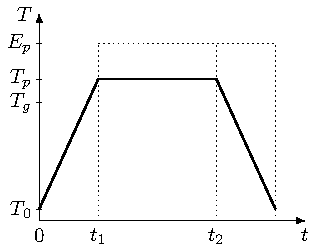
\includegraphics[width=0.4\textwidth]{tikz/coronapoling}\label{f:cp}} &
%\subfloat[]{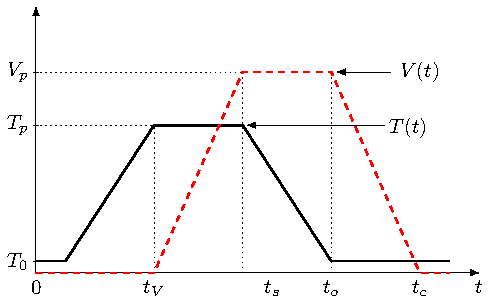
\includegraphics[width=0.5\textwidth]{tikz/corona-poling_ALL}\label{f:cpA}} \\
%\end{tabular}
%\caption{Schematic representation of corona poling. \ref{f:cp} shows only temperature, while \ref{f:cpA} shows also voltage and %current applied to the sample. Adapted from\cite{singhmiyataNLOorganic96}.}
%\label{fig:cpol}
%\end{figure}

%\begin{figure}[!ht]
%  \includestandalone[width=0.4\textwidth]{tikz/coronapoling}
%  \centering
%  \caption{Schematic representation of corona poling. $E_p$=Poling field, $T_p$=poling temperature, $T_g$=glass transition temperature, and $T_0$=room temperature. Adapted from \cite{singhmiyataNLOorganic96}.}
%  \label{fig:coronapol}
%\end{figure}

%for which $E_p$=Poling field, $T_p$=poling temperature, $T_g$=glass transition temperature, and $T_0$=room temperature


%\begin{enumerate}
%\item The sample is heated from room temperature $T_0$ to poling temperature $T_p$ and kept at constant temperature and pressure %inside a vacuum chamber.
%\item An external poling voltage $V_p$ (dashed line) is applied at time $t_V$ to the sample, generating a poling field $E_p$%\footnote{The poling field is not shown but it can be extrapolated from the sample width and voltage applied}.%
%\item The sample is cooled to room temperature at time $t_s$ after poling and the electric field is slowly ramped down. 
%\item The thermoelectric treatment generates an electret\footnote{Electrostatic analog of a magnet.}.
%\end{enumerate}

%The corona discharge is a partial breakdown of air at atmospheric pressure, and it is induced by the inhomogeneous electric field around the needle. 
%The corona ions have very low lateral conductivity, so only charges can leak during contact poling.
%Polymers can be crosslinked in order to improve stability over large ranges of temperature, at a set temperature.
%The charge distribution in electrode poling is uniform, but it allows for weaker electric fields than corona poling \cite{singhmiyataNLOorganic96}. 
%no idea what fast charging process is in this context
The electrode poling technique is advantageous because of the simplicity of the setup. The process uses a few volts (and a current within \SI{2}{\nano\ampere} to avoid electric degradation) \cite{BlumPoling98}. The poling technique in-plane gives a large nonlinear coefficient in the TE configuration due to field alignment. The molecular shape and guest-host interactions give the order parameters of a chromophore if there is no preferential orientation (i.e. it is randomly distributed).  Once crosslinking occurs at a specific temperature and the shape can no longer be changed the material is called a thermoset.  %Some crosslinked  polymers change their shape with temperature and cannot dissolve in solvents due to covalent bonding, leading to gelification. This can be overcome by using ionomers which have reversible crosslinking making them suitable for dynamic temperature situations. %By using an angle $\theta$ with respect to the laboratory reference axis, which has a Boltzmann distribution (given by dichroism and electronic distribution).

%Some interesting features can be observed in figure \ref{fig:coronapol}. The poling current behavior follows a $t^{-n}$ dependence \cite{BlumPoling98}

%%%%%%%%%%%%%%%%% Definition of crosslinking
%gelification is a word? 

\subsubsection{Organic material stability}

\begin{figure}[!ht]
\centering
\includestandalone[width=0.5\textwidth]{tikz/temp_dependence_volume_bosshard}
\caption{Temperature dependence of specific volume $V_{sp}$ near $T_g$ from Bosshard, et. al. \cite{BosshardOrgaNLO95}. The cooling parameter $q_1$ shows a linear and a nonlinear (dashed line) cooling rate depending on the properties of the polymer. The phase of the polymer is observed as glass (blue hatched area) and liquid (red hatched area). $T_{eq}$ shows the equilibrium temperature, $T_g$ shows the glass transition temperature and $T_m$ shows the melting temperature.}
\label{fig:Bosshard_temp}
\end{figure}


At high temperatures (above $T_m$, or melting temperature), the organic material is at liquid state (first order transition), with a thermal expansion coefficient (the slope of volume and temperature) $\alpha_l$, and a true equilibrium point at $T_{eq}$ with smaller thermal expansion coefficient $\alpha_g$. The actual phase transition occurs at the glass temperature $T_g$ where the liquid and glass states intersect (i.e. amorphous chain of molecular clusters), and is a kinetic phenomena that depends on the \textbf{cooling rate} $q$ as seen in figure \ref{fig:Bosshard_temp} \cite{BosshardOrgaNLO95}, which shows the measure of the specific volume with respect to temperature. The cooling rate curves are read from a high temperature (above the melting temperature) towards lower temperatures. A cooling rate $q_1$ which is larger than $q_2$ is also shown as well as nonlinear cooling rates, but still the glass temperature point is observed when there is an abrupt change of the thermal expansion coefficient. 

%At $T_g$ the free volume describes the polymer relaxation process, where the total volume is the sum of the free and occupied volumes $v= v_f+v_o$. %$v_o$ is given by the van der Waals radii including the volume associated with vibrational motions. In order to allow movement of molecular segments from one site to another, a critical volume $v_{cf}$ is needed. Considering that liquid expansion of a liquid over the glass state is caused by a thermal expansion coefficient and the free volume at glass transition temperature, 
%A dipolar relaxation time $\tau$ can describe segmental mobility, $r \propto \tau^{-1}$ the WLF equation describes the superposition parameter $a_T$\cite{BosshardOrgaNLO95}.:

%\begin{align}
%log a_T \equiv log \frac{\tau_T}{\tau_\text{ref}} = \frac{-C_1(T-T_\text{ref})}{C_2+(T-T_\text{ref})}
%\end{align}

%Describing also the behavior of viscosity and time-temperature shift factors, with ``universal'' fitting constants \footnote{in the literature it is always suggested to use the fitting parameter at a specific temperature from viscosity measurements} $C_1$ and $C_2$ with typical values for polymers of 17 and 52K. The Vogel-Fulcher formula \cite{BosshardOrgaNLO95}

%\begin{align}
%\tau = A^* e^{B/T-T^*} =  A^* e^{B/T-T_\text{ref} - C_2}
%\end{align}
%(and below $T_g$+\SI{100}{\kelvin}),
At temperatures close to $T_g$, stable behavior of the polymer can be achieved, by heating slightly above the glass transition temperature $T_g$, where maximum mobility of the optical guest molecules occurs. The anisotropy can be fixed by cooling down the polymer with the poling field still on. The shrinking of the specific volume reduces the free space for relaxations of the aligned moieties. This is of special interest to the integration process because the organic polymer is extremely sensitive to temperature, so special care must be taken in the order in which the materials are processed to reduce material instability that will result in overall bad device performance.


%\begin{figure}[!ht]
%\centering
%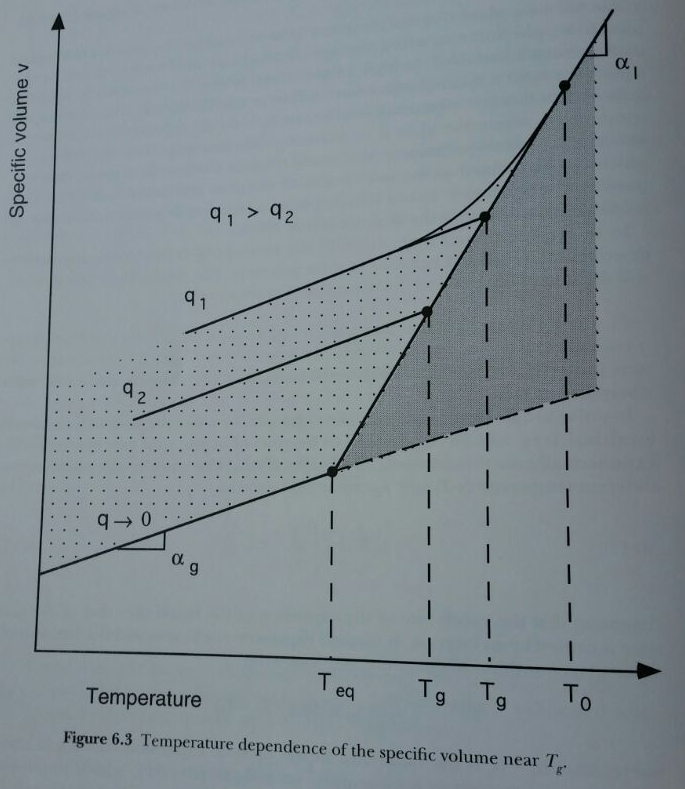
\includegraphics[width=0.7\textwidth]{figs/BosshardTempDependenceSpecificVolumeNearTg}
%\caption{CORRECT THIS BEFORE PRINTINGGGGG!°!!!!! Temperature dependence of specific volume near %T_g% from Bosshard, et. al.%\cite{BosshardOrgaNLO95}.}
%\label{fig:BehfarRidge}
%\end{figure}

%\section{Solvents (not needed probably)}
%\label{sec:OECompounds:Solvents}

%From wikipedia
%Isopropyl alcohol dissolves a wide range of non-polar compounds. It also evaporates quickly, leaves nearly zero oil traces, compared to ethanol, and is relatively non-toxic, compared to alternative solvents. Thus, it is used widely as a solvent and as a cleaning fluid, especially for dissolving oils. Together with ethanol, n-butanol, and methanol, it belongs to the group of alcohol solvents.

%Auch von wikipedia
%In the semiconductor industry, PGMEA is a commonly used solvent, primarily for the application of surface adherents such as Bis(trimethylsilyl)amine (HMDS) on silicon wafers.

%from http://www.chemicalland21.com/industrialchem/solalc/1-METHOXY-2-PROPYL%20ACETATE.htm

%They may be classified as polar and non-polar. Polar solvents, like water, have molecules whose electric charges are unequally distributed, leaving one end of each molecule more positive than the other. Usually polar solvent has O-H bond of which water (HOH), (\ce{CH3OH}) and acetic acid (\ce{CH3COOH}) are examples. Propanol, butanol, formic acid, formamide are polar solvents. Polar solvents are hydrophilic but non-polar solvents are lipophilic. Polar reactants will dissolve in polar solvents. Non-polar solvents dissolve non-polar compounds best. Oil and water don't mix but separate into two layers. There are three measures of the polarity as "dipole moment", "dielectric constant" and "miscibility with water". Though low dipole moments and small dielectric constants indicates non-polar solvents, sharp boundaries between polar and non-polar solvents are not available. The polarity reflects the balance between a polar component (OH) and a non-polar hydrocarbon component, existing in the same molecule. If hydrocarbon character increases relatively, the polarity decreases. On an operational basis, solvents that are miscible with water are polar.

%\textbf{The appropriate solvent should be selected based on the inactivity in the reaction conditions, dissolving the reagents as well as reactants, appropriate boiling point and easy removal at the end of the reaction.}

%\dots

%\section{Information Theory}
%\label{sec:InfoTheory:InfoTheory}

%\begin{figure}[!ht]
%  \includestandalone[width=0.3\textwidth]{tikz/gaussianchannel}
%  \centering
%  \caption{The Gaussian channel. Adapted from \cite{ThomasInfoTheory91}.}
%  \label{fig:gaussianchannel}
%\end{figure}

%%%%%%%%%%%%%%% RANDOM BOSSHARD QUOTES




%% ---------------------
%% | / Example content |
%% ---------------------


%\section{Solvents and Material Processing}
%\label{sec:solv:solvs}
%Wu states that "Water-soluble polymers can form hydrogels aftercrosslinking. The hydrogel is usually insoluble, butcan absorb considerable water and swell. The swelling ratio [...] strongly depends on the intrinsic properties of corresponding linear polymer, such as solubility and conformation. High solubility and ex-panded conformation in certain solvents lead to a high swelling ratio." \ref{Wu_Solv04}



%\subsection{Organic Electro-Optical Material Characterization}
%\label{sec:EO_optim}

%\lasnotas{probably not necessary}

%It is common to find much higher $r_{33}$ coefficient materials in the literature in very specific laboratory conditions, with comparable coefficients to \ce{LiNbO3} in dedicated SOH structures. In order to characterize electro-optical crystals the half-wave voltage $V_\pi$ is an important parameter, as it indicates the voltage required to obtain a $pi$ phase shift in the transmitted beam in a modulator:

%\begin{align}
%V_\pi = \frac{\lambda}{(n^3r)_\text{eff}\frac{d}{L}=v_pi \frac{d}{L}} 
%\end{align}

%With $(n^3r)_\text{eff}$ being the effective electro-optic coefficient. 




%% LaTeX2e class for student theses
%% sections/content.tex
%% 
%% Karlsruhe Institute of Technology
%% Institute for Program Structures and Data Organization
%% Chair for Software Design and Quality (SDQ)
%%
%% Dr.-Ing. Erik Burger
%% burger@kit.edu
%%
%% Version 1.2, 2016-09-20

%\chapter{Modulators and Waveguides}
%\label{ch:MW}

%In this chapter some elements of modulators and waveguides are provided. In many cases results are only provided instrumentally as they are not the focus of study in the present work, but references for further theoretical foundations are provided.
\clearpage
\section{Photonic Wire Bonds}

Photonic wire bonds (PWB) are optical waveguides based on polymers that interconnect different chips, much like wire bonding being a standard electrical connection technique in electrical integrated circuits. The PWB has a rectangular cross section of $\SI{1.4}{\micro\meter} \times \SI{1}{\micro\meter}$ which satisfies single-moded operation \cite{ToepferPWB14}.

\begin{figure}[!ht]
\centering
  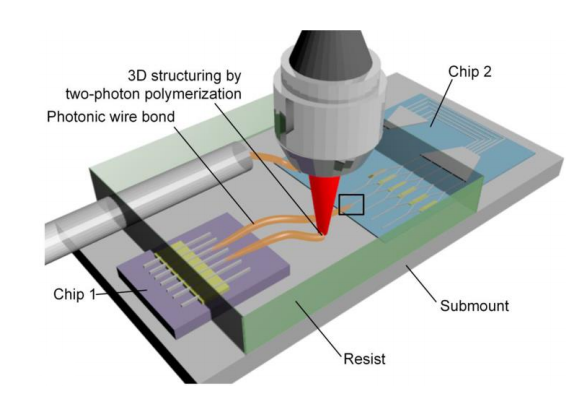
\includegraphics[width=0.6\textwidth]{figs/PWB_fab}
  \caption{Fabrication of PWB, illustrating the process of the connection. Two physically separated chips are placed in common submount, and a negative photoresist is added between the devices. Laser light polymerizes the photoresist by two-photon absorption. Adapted from \cite{ToepferPWB14}.}
  \label{fig:PWB_fab}
\end{figure}

As any other optical path, PWBs introduce losses due to material, bending and transition losses. The polymer losses account for \SI{3}{\decibel / \centi\meter} for $\lambda=\SI{1550}{\nano\meter}$; while bending losses are entirely path-dependent, they can be dynamically calculated when the PWB is written, while in general small curve radii most be avoided when writing PWB; Results from T{ö}pfer suggest a loss of \SI{0.24}{\decibel/\micro\meter} \cite{ToepferPWB14}. 

The material of which PWBs are made of is the negative-tone photoresist IP-Dip produced by Nanoscribe, catered for immersion and drop-casting processing. As any other polymer, the photonic wire bond should have a number of properties that match the pre- and post-processing of a multi-chip package, being the key properties \cite{PolyWong13}:

\begin{itemize}
\item \textbf{Optical properties:} The polymer must have a refractive index that allows for strong waveguiding with low losses. Additionally an overcoating can be used to match the refractive index and reduce return losses due to Fresnel reflections.
\item \textbf{Thermal properties:} The glass transition temperature must be high enough that the material will be stable over the range of temperatures in which the multi-chip module is processed. 
\item\textbf{ Mechanical properties:} The polymer used for the PWB must have a low thermal coefficient of expansion such that, throughout the many processes of the multi-chip module, there will be no warping or delamination of the PWB.
\item \textbf{Solvent resistance:} When the PWB is developed it should withstand different solvents used to remove the regions that are not polymerized. This also introduces a strain due to drying, which can be externally controlled by methods such as critical point drying to avoid uneven strain in the PWB.
\end{itemize}

%presents a glass transition temperature, which has to be taken into account during the thermal processing during device integration. 
The characterization of the PWB is done by measuring the optical paths available on-chip in which there is a well-known optical path. The SOH chips used throughout this master thesis have independent optical paths which allow for independent measurement of the transmission through the input or output PWB and grating couplers for measuring the transmission of the modulator only. The details of the measurement are provided in section \ref{sub:OPL}.

%\section{Photonic Wire Bonds}
\subsection{Fabrication Process}
\label{ch:th:fabPWB}

\begin{figure}[!ht]
\centering
  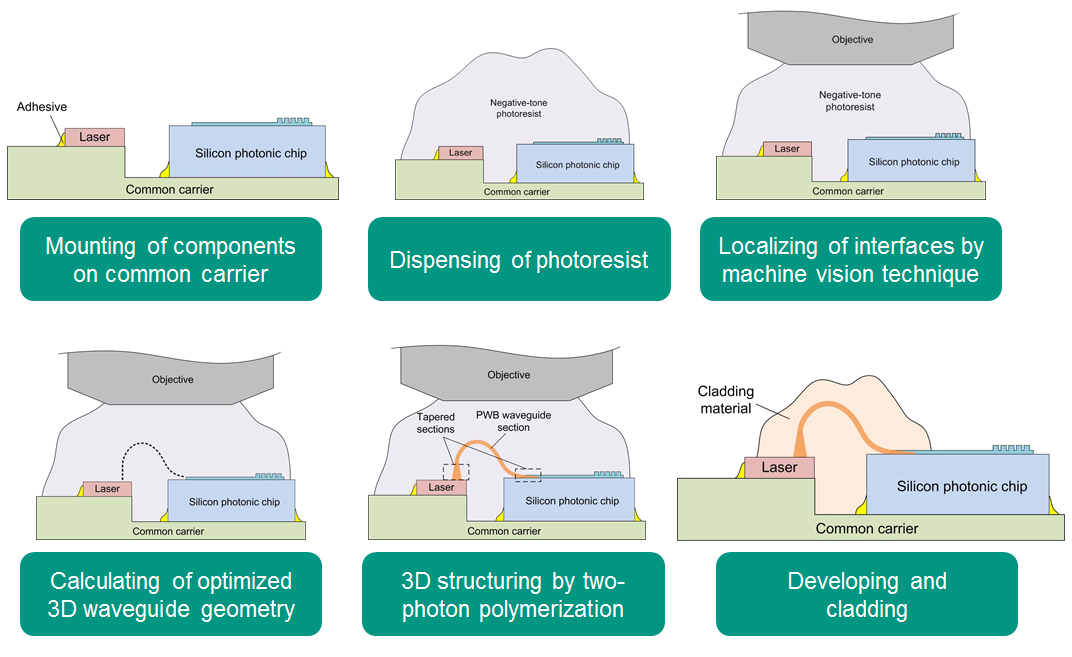
\includegraphics[width=0.9\textwidth]{figs/pkgprocess}
  \caption{PWB fabrication steps.}
  \label{fig:SOHpkg}
\end{figure}

Photonic wire bonds are not necessarily symmetric in a device since the path it follows depend on the location of the chips, especially when the processing of the chip is done manually. Nonetheless, the chip alignment is not as critical when the dimensions of the chips and components is well known and can be controlled prior to the writing of the PWB. and just determines the losses of the PWB. The fabrication process of the photonic wire bonds is illustrated in figure \ref{fig:SOHpkg}:

\begin{enumerate}
\item The components are placed on top of a common carrier, fabricated in-house, made with aluminum. The components are passively aligned by hand and glued with thermally-curable epoxy. 
\item The IP-dip photoresist is dispensed on top of the common carrier, making sure there is enough photoresist in the region of interest (i.e.between the SOH and the HCSEL).
\item The module is placed in the printing machine and the position of the HCSEL and SOH is found using the software. The structures on-chip that allow for localizing the emission window, tapers and fibers.
\item The waveguide structure is calculated based on the chip distance, relative height, and after inspecting the geometry as a 3D model, the final shape is selected.
\item The PWB is written by polymerization of the IP-dip through two-photon absorption. 
\item After all the required PWB are written, the PWB is developed and prepared for local deposition of the electro-optical polymer.
\end{enumerate}

\subsection{Photonic Wire Bond Stability}

\begin{figure}[!ht]
\centering
  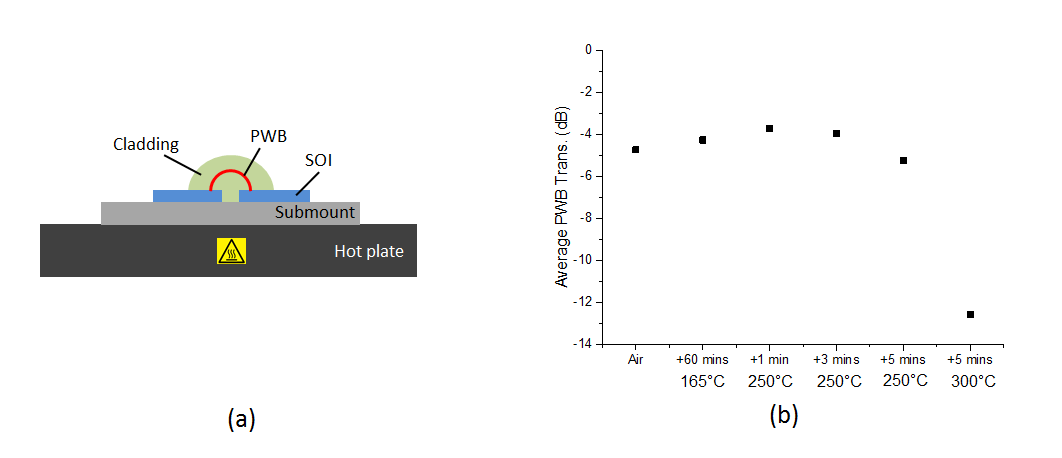
\includegraphics[width=0.9\textwidth]{figs/PWB_stab}
  \caption{PWB stability test. (a) shows the setup, consisting of a hot plate used to control the temperature of the metallic submount in which an SOI is integrated with an overcladded PWB. Figure (b) shows the average PWB transmission in dB for different temperatures and conditions. A standard control measurement in air is taken, and different temperature steps and thermal exposure times are also pictured.}
  \label{fig:SOHtherm}
\end{figure}

The thermal and mechanical stability of the photonic wire bond are of great importance during the integration process since it determines the reliability of its function throughout the lifetime of the optical transmitter. Such study has been addressed by doing thermal stability testing on a functional PWB in a test structure as shown in \ref{fig:SOHtherm}. The setup is a simple hot plate that controls the temperature of a mounted SOI/PWB combined chip, and the transmission on-chip is measured after thermal exposure of the chip. The PWB retains a stable transmission at thermal exposure of more than 60 minutes at \SI{165}{\celsius} and more than 5 minutes at a temperature \SI{250}{\celsius}, thus the reliability of the PWB under laboratory conditions is confirmed for temperatures up to \SI{250}{\celsius}. Further application of heat reaches the glass transition temperature of the IP-dip polymer, which in affects its mechanical stability and causes collapsing of the PWB (thus losing the intended optical path) or in the worst case scenario, detachment from the tapers and inoperability of the device.



\section{Integrated Transmitters}

Even though optical modulation can be done directly in some laser diodes, the most reliable method at high transmission speeds is still external modulation, since it provides with larger degrees of freedom in terms of chirp control, bandwidth and distortion \cite{WootenLiNBo300}. 

The integration of the optical modulator to the optical source is of crucial importance in the miniaturization of devices, since the dimensions of each must be mutually matched in order to accommodate mechanically in a shared common carrier. 

%\subsection{Figures of Merit}
\subsection{Horizontal Cavity Surface Emitting Laser} 

In order to create a semiconductor laser, a resonator structure must be integrated into a very small form factor. To achieve this, a distributed Bragg reflector (DBR) can be used, which consists of a stack of waveguides, in which several partial reflections of an optical wave occur. This leads to a selective photonic passband and thus, acting as the optical cavity of a laser. In order to allow for optical confinement, two n- and p-doped semiconductor layers acting as mirrors are added to an optically active layer, which is known as an \textbf{edge-emitter laser}. If an additional mirror is added at the emission window, and total reflection occurs, the laser beam is emitted vertically, and thus, the basic structure of a horizontal-cavity, surface emitting laser (HCSEL) is achieved \cite{Eichlerlaser15}. %Additionally they are easy to test and package and build. 


%BH_LO_Swingler
\begin{figure}[!ht]
\centering
\begin{tabular}{cc}
\subfloat[Vertical cross-section adapted from \cite{SwinglerThermal14}]{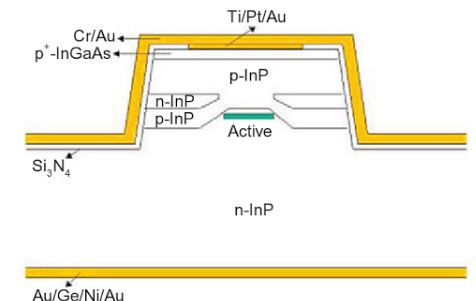
\includegraphics[width=0.4\textwidth,valign=m]{figs/BH_LO_Swingler}\label{fig:RidgeSwingler}} &
\subfloat[Horizontal cross-section adapted from \cite{MoehrleHCSEL10}]{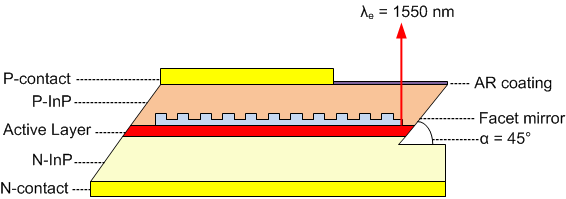
\includegraphics[width=0.5\textwidth,valign=m]{visio/HCSEL_LO}\label{fig:HCSEL_LO}}  \\
\end{tabular}
\caption{HCSEL structure and stack-up.(a) shows a vertical stack-up of a typical InP-based buried heterostructure, featuring conductive metallic layers at the bottom for electrical interconnections, and several InP n- and p-doped layers surrounding the active region at the core of the heterostructure, (b) shows a horizontal stack-up showing details of the active layer and gratings used, as well as the location of the outcoupling mirrors and the contact types. }
\label{fig:HCSELdims}
\end{figure}

%\begin{figure}[!ht]
%\centering
%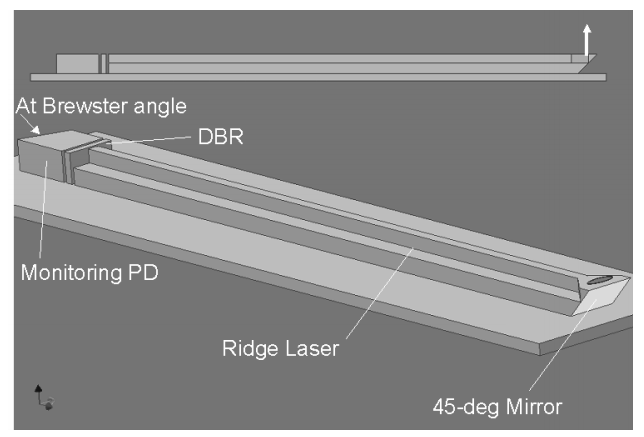
\includegraphics[width=0.7\textwidth]{figs/Ridge_fromBehfarHCSEL05}
%\caption{Cross-sectional and perspective views of a HCSEL, taken from Behfar, et. al.\cite{BehfarHCSEL05}.}
%\label{fig:BehfarRidge}
%\end{figure}

%\begin{figure}[!ht]
%\centering
%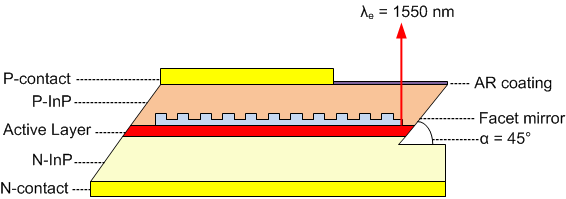
\includegraphics[width=0.6\textwidth]{visio/HCSEL_LO}
%\caption{HCSEL stack-up, adapted from \cite{MoehrleHCSEL10}.}
%\label{fig:HCSEL_LO}
%\end{figure}

The work of Behfar \cite{BehfarHCSEL05} and Moehrle \cite{MoehrleHCSEL10} for the structural and specific dimensioning of the HCSEL were used as a reference for this thesis. A ridge waveguide structure is used for the confinement of light in the lateral region, because of the slight change of the refractive index under the ridge with respect to the etched part, thus achieving weak guiding. Strong guiding structures are not usually used because the edges of the optical core can be actively damaged by a deep etch. Narrow ridges are used for single-lateral mode operation and to the mode matching of the laser to the waveguide \cite{ZappeLaser04} (in this case, the size of the PWB).  The \SI{45}{\degree} angle prevents the ridge structure from interfering with the beam shape \cite{BehfarHCSEL05}. Figure \ref{fig:HCSEL_LO} shows the stack-up structure of a HCSEL buried structure. The HCSELs used in this master thesis are multi-quantum well \ce{InP}. For the emission window, \SI{45}{\degree} facet mirrors are used to emit light vertically.  %An additional monitoring photodector is added after the DBR for power metrology, and it features a Brewster angle-cut facet to avoid back reflections \cite{BehfarHCSEL05}.%Not necessary to talk about the monitoring photodetector
%Analysis

%In order to obtain the dimensions of the laser, a reference image is used from the first SEM pictures and using the image processing software ImageJ. \ref{fig:HCSELdims} shows the approximate dimensions of the ridge waveguide made for the HCSEL. 

\begin{figure}[!ht]
\centering
\begin{tabular}{cc}
{\subfloat[SEM picture]{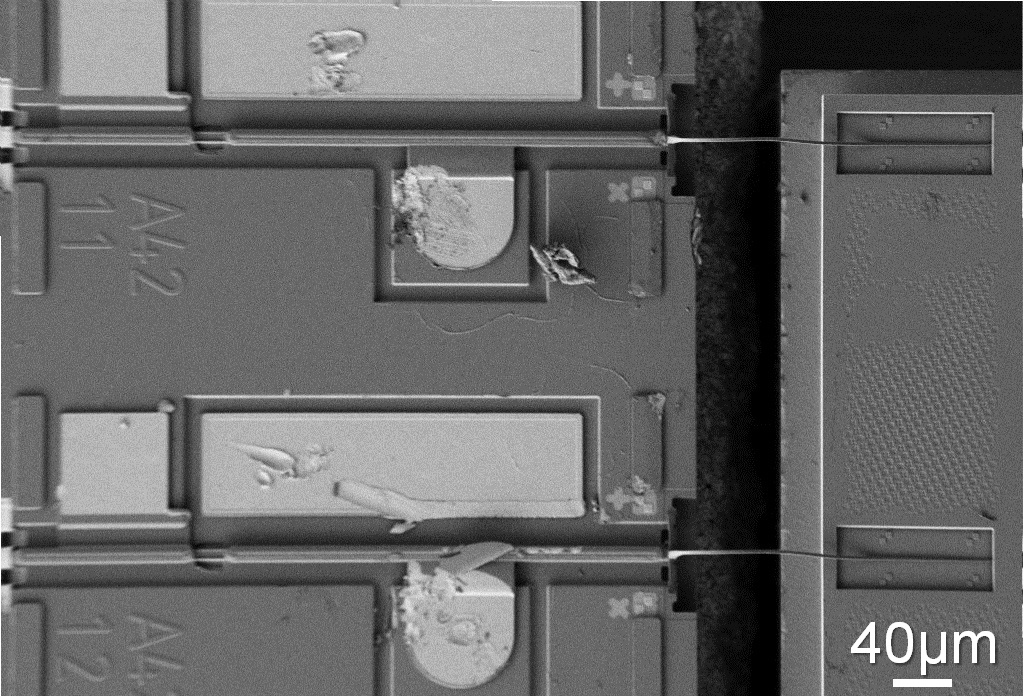
\includegraphics[width=0.4\textwidth,valign=m]{SEM/laser_MCM01}\label{SEMlaser}}} &
{\subfloat[Schematic dimensions]{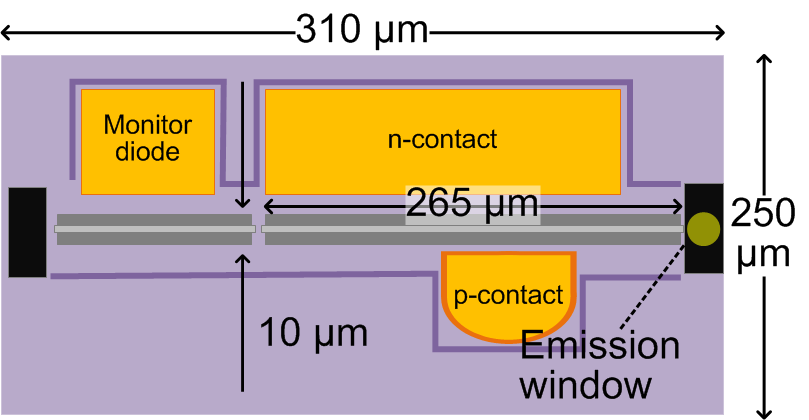
\includegraphics[width=0.5\textwidth,valign=m]{visio/HCSEL-dim_v2}\label{HCSELdim}}}  \\
\end{tabular}
\caption{HCSEL dimensions. \ref{SEMlaser} shows the SEM image of the HCSEL. \ref{HCSELdim} shows the image analysis-calculated dimensions from the SEM picture.}
\label{fig:HCSELdims}
\end{figure}

The HCSELs are packaged in arrays of four units. In general, an array of 2 HCSEL arrays (total 8 units) was tested for MZM modulators, while a single HCSEL array was sufficient for IQ modulators. In order to measure quantitatively the performance of a HCSEL array, one expects it to behave predictably at a specific temperature with a constant output power, high side mode suppression ratio and single longitudinal mode operation. Depending on the level of maturity of the laser, the characterization properties are changed in priority with respect to their importance at the system level.
%What limits the maximum output power of ong wavelength InP laser diodes
%verbatim! from  http://citeseerx.ist.psu.edu/viewdoc/download?doi=10.1.1.589.9034&rep=rep1&type=pdf
%for my laser !!!!!strain compensated MQW InGaAsP/InP layer structure!

\subsubsection{Laser Requirements}

The L–I roll-off is typical for laser diodes and it is attributed to self-heating of the device in CW operation. Temperature elevation affects a number of key physical mechanisms in laser diodes, including the optical gain, optical losses, and nonradiative recombination mechanisms [find citation here]. 

In order to use high order modulation formats (as those used in IQ modulators, for example), the laser linewidth has an increasingly important role. In a time period $\tau$, the laser phase noise has a change of $\Delta \phi(t)= \phi(t) - \phi(t-\tau)$  and variance $\left< \Delta\phi^2(t) = 2\pi(\Delta \nu \tau) \right>$, where $\Delta\nu$ is the laser linewidth. Thus, if the laser phase noise variance depends on the laser linewidth, any small phase variations coming from the laser source will affect the constellation distribution in the modulator. The work of Seimetz \cite{SeimetzLaser08} analyzed through Monte Carlo simulations the maximum tolerable linewidth, with $\Delta \nu=\SI{10}{\mega\hertz}$ for QPSK and $\Delta \nu=\SI{120}{\kilo\hertz}$ for square 16QAM (and intermediate values for the remaining modulation formats between the aforementioned examples) at \SI{40}{\giga bit/\second} for a maximal receiver sensitivity penalty of \SI{2}{\decibel} at a bit error probability of \SI{1e-4}{}. This provides a good rule of thumb of the expected linewidth of the laser sources used in an integrated modulator.

The laser linewidth, while detrimental in some cases, is not always an avoidable trait of an optical transmitter. For this reason, other methods can be used to circumvent around the laser linewidth limitation. One such method is the Kalman filter phase tracking, which implement a predictor-corrector type of estimator optimized for the estimated error covariance based on linear minimum mean square error (LMMSE). Its advantages are that it applies with stationary and non-stationary models and it is based on state space modeling \cite{AcunaPnoise13}. 

\subsubsection{HCSEL Pre-characterization}

 The parameters of largest importance in optical integration can be assessed in the following according to \cite{HertsensLD05}:

\begin{itemize}
\item \textbf{Electrical characterization:} The illumination provided by a laser diode, which is detected by a photodiode receiver (or an integrating sphere), is directly proportional to the power injected to the laser diode, which is dependent of the injection current and the correlated temperature and voltage drop in the junction. A light-current (LI) curve provides information on critical points, such as threshold current and maximum operation current. It also provides information on potential thermal roll-off, which occurs when the maximum light output power reaches its maximum before the operation current and decreases steadily afterwards, can also be observed with this measurement, as well as non-monolithic power curves. 
\item \textbf{Spectral characterization:} Single mode operation can be affected by mode hopping, which depends again on temperature and injection current. Even if a laser diode is designed for single mode operation, other modes can appear and modify the spectral properties of the laser, thus changing the pulse shape and step response of the output of the laser. A current sweep provides information on potential mode-hopping, spectral hole burning, and any other observable spectral features.
%\item \textbf{Dynamic characterization:} Relative intensity noise (RIN) is a highly frequency-dependent noise source, having separate components: shot noise is observed at very high frequencies, \lasnotas{while at low frequencies noise from the injection current are observed [?, check source]}, and a strong peak due to damped relaxation oscillations in the lattice of the semiconductor. Other properties such as distortion, rise and fall time and chirping can be addressed in the dynamic operation characterization.
%\item \textbf{Linewidth characterization:} Once a single mode operation is achieved, the linewidth of the laser provides an indication of the coherence properties of the laser. This can be measured through self-heterodyne detection\footnote{this provides a simple self-convolution of the laser output spectrum} , which provides the spectral coherence of the laser diode. 
\end{itemize}


\begin{figure}[!ht]
\centering
\begin{tabular}{cc}
\subfloat[LI Curve]{\includestandalone[width=0.4\textwidth]{tikz/LIcurve}\label{licv}} &
\subfloat[Spectrum]{\includestandalone[width=0.4\textwidth]{tikz/spectrum}\label{scv}} \\
%\subfloat[]{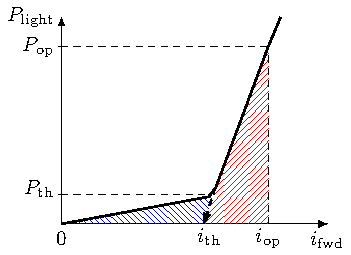
\includegraphics[width=0.4\textwidth]{tikz/LIcurve}} &
%\subfloat[]{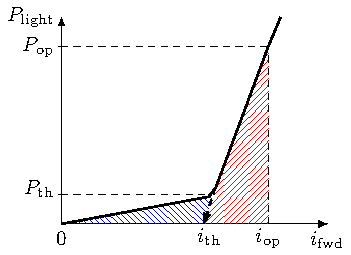
\includegraphics[width=0.4\textwidth]{tikz/LIcurve}} 
\end{tabular}
\caption{Typical characterization curves. (a) Shows the LI curve. Forward current $i_\text{fwd}$ is injected to a laser diode and spontaneous emission dominates (hatched blue area). At the threshold current $i_\text{th}$ stimulated emission dominates and lasing occurs. The operation current $i_\text{op}$ is the point at which the laser diode is typically biased in normal operation. (b) shows the spectral red shift of a laser diode as forward current is increased.}
\label{fig:charcv}
\end{figure}

Figure \ref{fig:charcv} shows some typical characterization curves that can be obtained experimentally. Figure \ref{licv} shows a typical output light-injected current (LI) curve. The northwest (blue) hatched area shows the spontaneously emitted light (before population inversion is achieved in the laser). The northeast (red) hatched area shows the laser light emission region (past threshold current $i_\text{th}$). The operation current $i_\text{op}$ and power $P_\text{op}$ are the typical operation points of the lasers in continuous wave (CW) mode. This curve provides information about the slope efficiency (light percentage proportional to current, in \SI{}{\milli\watt/\milli\ampere} units). Figure \ref{scv} shows a typical spectrum measurement for laser diodes. The spectrum is assumed to be Gaussian and the laser diode is above threshold ($i > i_\text{th}$). As the injected current is increased $i_1>i_2$, the spectrum of the laser diode will red-shift because the refractive index temperature dependence inside the laser cavity. In some cases, this red-shift can lead to more severe conditions such as mode hopping (i.e. adjacent longitudinal mode gain shift) which is not desirable in applications such as WDM where adjacent wavelengths can be affected by crosstalk of interfering channels.

%Second order non-linearities can be achieved in many 



\subsection{Full Transmitter}
\begin{figure}[!ht]
\centering
  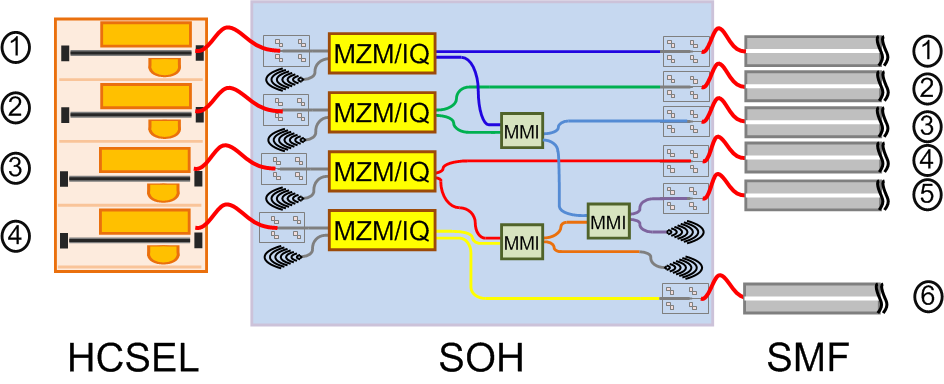
\includegraphics[width=0.9\textwidth]{visio/Concept}
  \caption{Conceptual schematic of an optically packaged transmitter. A HCSEL laser diode is connected through a PWB to an SOH MZM chip that modulates the laser light and output through a PWB to a single mode fiber. Grating couplers can be used to measure individual components in the SOH device. Combination schemes inside the SOH allow for wavelength division multiplexing (WDM) or parallel single mode (PSM) output.}
  \label{fig:concept}
\end{figure}

Figure \ref{fig:concept} shows a conceptual representation of such optically transmitted. An integrated laser is used as the optical source. The type of laser varies from application to application, but in general semiconductor laser diodes are used, with configuration such as vertical cavity surface emitting lasers (VCSEL) \cite{IntPWBPetek16}; discrete mode lasers (DML) \cite{SOHPajkovic16}; and in the present case, a horizontal cavity surface emitting laser (HCSEL). A photonic wire bond (PWB) connects both ends of the optical path, and it is written via direct laser writing (DLW). A Mach-Zender modulator mixes the optical and electrical signal, and in the most general case, it is combined by using multi-mode interferometers (MMI) and output again through a PWB into a single mode fiber (SMF). The whole device is then optically packaged by means of curable UV glue or another cross-linkable polymer to avoid damage to the PWBs and to allow for easier transport (at the cost of reduced debug capabilities, since the integrated grating coupler inputs and outputs are effectively disabled during the optical packaging process).
%\section{Integrated Modulators}

\subsubsection{Optical Path Loss}
  \label{sub:OPL}

The optical path loss or link budget provides information of the performance of an optical link. It is a useful figure of merit to compare the performance of optical links. In order to characterize individual links in the optical path, several measurements can be carried to isolate the power losses at each stage. Figure \ref{fig:OPL-flow} shows the schematic of the optical path from the laser generator (HCSEL or tunable laser source) to the output fiber.

\begin{figure}[!ht]
\centering
  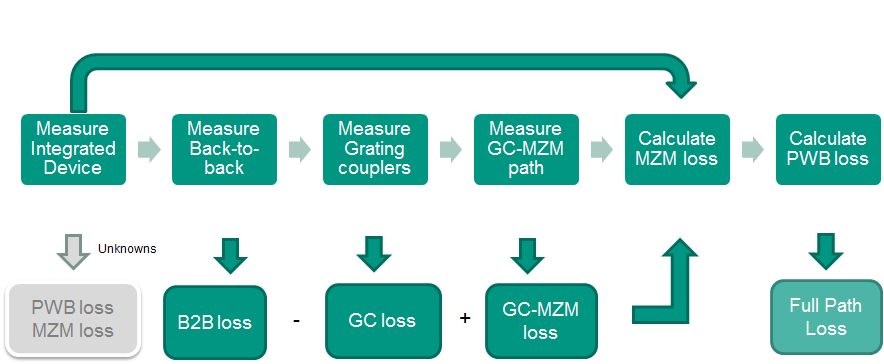
\includegraphics[width=0.8\textwidth]{visio/OPL-flow}
  \caption{Optical path loss calculation flow diagram.}
  \label{fig:OPL-flow}
\end{figure}

\begin{figure}[!ht]
\centering
  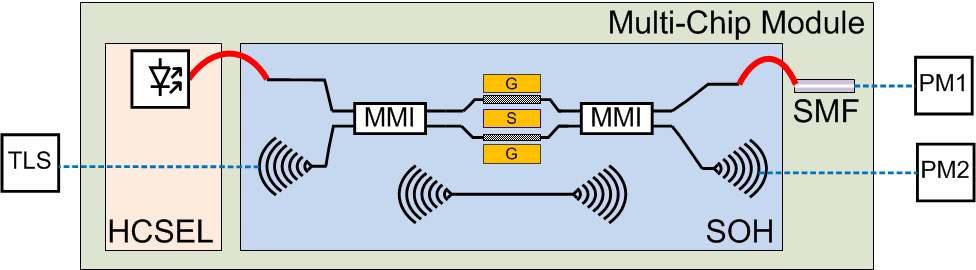
\includegraphics[width=0.8\textwidth]{visio/MCM-LO}
  \caption{Schematic setup for measuring optical path loss. As laser sources the integrated HCSEL and tunable laser sources (TLS) can be used. Light can be coupled through a PWB or a grating coupler. The output can be monitored with a grating coupler or the integrated single mode fiber through a PWB.}
  \label{fig:mcm-LO}
\end{figure}

%With the information for the operation point of the laser at \SI{75}{\milli\ampere}, 
The optical setup is arranged as in figure \ref{fig:mcm-LO} to measure the following optical paths:

\begin{itemize}
\item HCSEL $\rightarrow$ MZM $\rightarrow$ Output fiber
\item Tunable laser source (TLS) $\rightarrow$ Optical spectrum analyzer (OSA) (back-to-back)
\item Grating coupler (GC) $\rightarrow$ Grating coupler test structures (GC loss)
\item TLS $\rightarrow$ GC $\rightarrow$ MZM $\rightarrow$ GC $\rightarrow$ OSA (GC-MZM path)
\end{itemize}

These independent measurements can be combined to estimate the insertion loss of the MZM and the PWB by following the flow diagram as shown in \ref{fig:OPL-flow}. As mentioned earlier, the losses of the PWB are path-dependent so any path difference in the PWB path between the input and the output can change the loss distribution if measured as above. If the trajectories of the PWB are very pronounced, cross-transmission measurements can be done in addition to the former measurements:

\begin{itemize}
\item HCSEL $\rightarrow$ MZM $\rightarrow$ GC
\item TLS $\rightarrow$ MZM $\rightarrow$ SMF
\end{itemize}

Such measurement is of interest when the specific transmission characteristics of the input and output photonic wire bond need to be decoupled and the losses of a single photonic wire bond need to be characterized.